%% main.tex — ERL Letter submission
%% Journal: Environmental Research Letters (IOP, IF 6.7)
%% Format: Letter ~3000 words, 3 figures, 2 tables
%%
%% NOTE: iopart.cls stub provided for local compilation.
%% Replace with official iopart.cls (https://ctan.org/pkg/iopart)
%% and iopart-num.bst before final submission.

\documentclass{iopart}

\usepackage{amsmath}
\usepackage{graphicx}
\usepackage{booktabs}
\usepackage{hyperref}
% IOP uses numbered citations — natbib not needed with unsrt
% \usepackage[round]{natbib}

% For review: show line numbers
% \usepackage{lineno}
% \linenumbers

\begin{document}

\title{Pixel-Scale Deforestation Risk Prediction in the Congo Basin:%
\ A Feature Ablation Study Across Spatial Scales, Temporal Depths,%
\ and Information Dimensions}

\author{Guillaume Laugie$^1$\footnote{Corresponding author: [email]}
and Marc Bouvier$^2$}

\address{$^1$ Univ. Grenoble Alpes, CNRS, Grenoble, France}
\address{$^2$ NitiDae, Montpellier, France}

\begin{abstract}
Accurate prediction of deforestation risk at pixel scale is a prerequisite
for early-warning systems and targeted conservation interventions, yet the
relative importance of different information sources remains poorly
characterised, particularly in the data-scarce Congo Basin.
We present a systematic feature ablation study across three dimensions---
information type, spatial scale of neighbourhood context, and temporal
depth of lag encoding---applied to a 250\,000-pixel sample of Hansen
Global Forest Change data over Central Africa (tile 10°N/020°E, 2016--2024).
An XGBoost gradient boosted trees classifier is trained on a strict
forward-looking temporal split (training predicts 2020--2022,
validation predicts 2024) to avoid any form of data leakage.
The core finding is that \emph{spatial contagion}---the deforestation
rate measured within 150\,m to 5\,km of each pixel---is the dominant
predictive signal, outperforming demographic, climatic, and
economic variables by a substantial margin
(AUC-ROC 0.947 vs.\ $\leq$0.86 for all other single-group models).
Temporal depth beyond a single lag year provides marginal gain
($\Delta$AUC $<$0.003), revealing short-term stationarity in
deforestation dynamics. A four-radius buffer combination achieves
AUC-ROC~0.957 and PR-AUC~0.076 (baseline prevalence: 0.36\%), yielding a
23-fold lift over random screening at the 1\% threshold.
We discuss implications for operational monitoring and the limits
of governance and economic indicators as predictive features.
\end{abstract}

\noindent\textit{Keywords}: deforestation, Congo Basin, machine learning,
XGBoost, spatial contagion, feature ablation, early warning


% ===========================================================================
\section{Introduction}
% ===========================================================================

The Congo Basin harbours the world's second-largest contiguous tropical
forest and is critical for global carbon storage and biodiversity.
Yet it is undergoing accelerating tree cover loss, with annual deforestation
rates estimated at 0.2--0.4\% driven predominantly by small-scale
subsistence agriculture~\cite{Tyukavina2018, Shapiro2023}.
Unlike South-East Asian and Brazilian deforestation, which are concentrated
in large industrial clearings, Congo Basin forest loss is spatially
diffuse~\cite{Ernst2013, Potapov2012}, making remote-sensing-based
detection challenging but early-warning prediction particularly valuable.

Pixel-scale prediction of where deforestation will occur one to two years
ahead would allow NGOs, national forest agencies, and REDD+ programmes to
target patrolling and land-tenure interventions more efficiently.
The literature on machine learning for deforestation prediction
has grown substantially, encompassing random forests on tabular features,
convolutional neural networks on image patches~\cite{Ball2022, Irvin2024},
and, more recently, large pre-trained Earth-observation
models~\cite{Jakubik2024, ForestCast2025}.
Yet few studies have systematically decomposed predictive performance
to answer the practical question: \emph{which information sources
and encoding choices actually matter?}

Drivers of deforestation span multiple spatial and temporal scales.
Distance to roads and settlements determines access cost; land-tenure
and governance shape incentives~\cite{Busch2017, Hosonuma2012};
commodity prices influence opportunity cost at national scale
\cite{Pendrill2019, Ordway2017}; and local deforestation history
encodes a spatial contagion process by which cleared land attracts
further clearing at the forest frontier~\cite{FerrerVelasco2020}.
It remains unclear how these factors trade off in predictive power,
or whether the predictive signal is sufficiently stationary to be
captured with a short temporal window.

Here we address these gaps through a triple ablation experiment on
a 250\,000-pixel dataset spanning Central Africa (2016--2024).
We evaluate nine categories of predictor variables extracted from
thirteen open data sources via Google Earth Engine~\cite{Gorelick2017};
test four spatial scales for neighbourhood deforestation context
(150\,m, 500\,m, 1.5\,km, 5\,km radii); and vary temporal encoding
from one to four lag years.
All experiments use a strict forward-looking temporal split to ensure
that training data never overlaps with the validation forecast window,
a design criterion often violated in prior work~\cite{Roberts2017}.


% ===========================================================================
\section{Data and methods}
% ===========================================================================

\subsection{Study area and target variable}

The study area corresponds to the Hansen Global Forest Change
(GFC~v1.12)~\cite{Hansen2013} tile at 10°N/020°E, covering approximately
10° $\times$ 10° across the Democratic Republic of Congo, Central African
Republic, South Sudan, Chad, and Uganda (Figure~\ref{fig:study_area}).
We sampled 250\,000 pixels at 30\,m resolution using stratified random
sampling, oversampling forest pixels with recent loss history.
The binary target is $y=1$ if pixel $i$ experienced tree-cover loss
in year $t$ (the \emph{prediction year}), and $y=0$ otherwise,
as recorded in the Hansen \texttt{lossyear} band.

\subsection{Feature engineering and data sources}

For each pixel $i$ and each prediction year $t^*$, we extract
predictor features from the preceding $K$ years using a \emph{sliding
window} encoding.
Let $x_{i,t}$ denote the value of a time-varying variable for pixel $i$
in year $t$; three complementary representations are derived:
\begin{align}
  \text{(i)~lags:} &\quad x_{i,t^*-k}, \quad k = 1, \ldots, K, \label{eq:lags} \\
  \text{(ii)~differences:} &\quad \Delta x_{i,t^*-k} = x_{i,t^*-k} - x_{i,t^*-k-1}, \quad k = 1, \ldots, K{-}1, \label{eq:diff} \\
  \text{(iii)~window mean:} &\quad \bar{x}_{i,t^*} = \frac{1}{K}\sum_{k=1}^{K} x_{i,t^*-k}. \label{eq:wmean}
\end{align}
Because all representations use only values strictly before $t^*$,
no future information leaks into the features.
This encoding is applied to all time-varying sources;
the ablation over encoding schemes (Section~\ref{sec:results_temporal})
evaluates each representation individually and in combination.

Static or slowly-varying features are extracted once per pixel:
topography from the Shuttle Radar Topography Mission~\cite{Farr2007};
distance to the nearest road, settlement, and protected area from
OpenStreetMap~\cite{OSM2024}; and binary protected-area status from
the WDPA database enriched with IUCN governance categories.

Time-varying sources include:
multi-scale neighbourhood deforestation rates at 150\,m, 500\,m,
1.5\,km and 5\,km radii computed from the Hansen GFC raster
(the \emph{spatial contagion} features);
pixel-level cumulative forest loss;
annual population density from WorldPop~\cite{Tatem2017};
monthly precipitation from CHIRPS~\cite{Funk2015};
temperature, evapotranspiration, and soil moisture from
ERA5-Land~\cite{MunozSabater2021};
night-time light radiance from VIIRS~\cite{Elvidge2017};
MODIS active fire counts~\cite{Giglio2016};
and three global commodity prices (cocoa, palm oil, gold)
as proxies for economic pressure.
After sliding-window expansion, the full feature set comprises
up to 549 variables organised into the nine groups
listed in Table~\ref{tab:ablation}.

\subsection{Experimental design}

\paragraph{Temporal split.}
To evaluate true out-of-sample generalisation, we construct two
physically separate datasets: a training set with prediction years
2020--2022 (features from 2016 onwards; $N_\mathrm{train}=729\,114$,
$n^+_\mathrm{train}=2\,525$) and a validation set with prediction year
2024 (features from 2017 onwards; $N_\mathrm{val}=240\,230$,
$n^+_\mathrm{val}=871$, prevalence 0.36\%; training set prevalence is 0.35\%).
The training set never includes observations from 2023, which serves
exclusively as lag input for the 2024 validation.

\paragraph{Classifier.}
We use XGBoost gradient boosted trees~\cite{Chen2016} with early
stopping on the validation log-loss.
Class imbalance is handled by setting
\texttt{scale\_pos\_weight}$= \lfloor(N_\mathrm{train} - n^+_\mathrm{train}) /
n^+_\mathrm{train}\rfloor = \lfloor 726\,589 / 2\,525 \rfloor = 288$,
matching the negative-to-positive ratio in the training set.
Hyperparameter tuning was performed using Bayesian optimisation
(50 trials, Optuna~\cite{Akiba2019}) minimising validation log-loss;
the tuned configuration was then retrained on the full training set.
No spatial or temporal cross-validation is applied during training;
all generalisation claims are based on the held-out 2024 forecast.

\paragraph{Ablation experiments.}
We conduct three sets of ablation experiments.
\emph{Dimensional ablation}: each of the nine feature groups is used alone,
and groups are then added cumulatively in decreasing order of
single-group AUC.
\emph{Spatial ablation}: the four buffer radii are evaluated in selected
pairwise combinations and as a full set.
\emph{Temporal ablation}: window depth is varied from $K=1$ to $K=4$ years,
and four encoding schemes are compared (lags only; lags + summaries;
lags + differences; full encoding).

\paragraph{Evaluation metrics.}
For severely class-imbalanced predictions, area under the
precision-recall curve (PR-AUC) is a more discriminating metric
than AUC-ROC~\cite{Mayfield2017}.
We report both throughout and complement them with two
operationally interpretable quantities.
The \emph{concentration curve} $C(s)$ is defined as the fraction
of total positive events recovered by screening the $s$ fraction
of pixels with the highest predicted risk; it summarises the model's
ability to concentrate deforestation risk into a small target area.
\emph{Lift} at screening fraction $s$ is defined as
$\mathcal{L}(s) = \mathrm{recall}(s)/s$,
where $\mathrm{recall}(s)$ is the fraction of positive events
recovered by screening the top-$s$ fraction of pixels;
a lift of 23 at $s=0.01$ means the model finds 23 times more
deforestation events per unit area than random selection.

\paragraph{Interpretability.}
TreeSHAP~\cite{Lundberg2017, Lundberg2020} is used to attribute
model predictions to individual features, enabling identification
of the dominant predictive mechanisms.


% ===========================================================================
\section{Results}
% ===========================================================================

\subsection{Dimensional ablation: spatial contagion dominates}

Table~\ref{tab:ablation} summarises the performance of each feature group
in isolation.
The spatial contagion group achieves by far the highest single-group
performance (AUC-ROC 0.947, PR-AUC 0.051 with 100 features), followed
at a substantial distance by infrastructure access (AUC 0.858, 12 features)
and population density (AUC 0.832, 13 features).
Local Hansen deforestation history without neighbourhood context yields
AUC 0.792, confirming that the landscape-scale signal---where is the
deforestation frontier?---is more informative than the pixel's own past.
Economy (commodity prices, governance indices, WDI) performs no better
than chance (AUC 0.500), a result we discuss in
Section~\ref{sec:discussion}.

Cumulative combinations show rapid saturation.
Combining spatial contagion features with Hansen local history
already reaches AUC 0.955, PR-AUC 0.075 (127 features).
Adding infrastructure access produces the optimal configuration
(AUC 0.955, PR-AUC \textbf{0.076}, 139 features; hereafter
the \emph{core model}).
Beyond this core, adding population, climate, NTL, and economic features
leaves AUC unchanged while PR-AUC decreases from 0.076 to 0.068.
This pattern is consistent with noise dilution in the minority class:
adding features that are weakly correlated with the target increases
the variance of tree splits without improving signal, causing the
boosted ensemble to fit spurious patterns in the positive class and
thereby degrading precision at high recall thresholds.
AUC-ROC is less sensitive to this effect because it evaluates ranking
globally across both classes, whereas PR-AUC weights errors in the
rare positive class more heavily.

\begin{table}[htb]
\caption{\label{tab:ablation}
Dimensional ablation: validation performance by feature group
(sorted by single-group AUC-ROC).
Cumulative results show the core model (Hansen + Spatial + Infra)
as the optimal configuration.}
\begin{center}
\begin{tabular}{lrll}
\toprule
Feature group & $N_\mathrm{feat}$ & AUC-ROC & PR-AUC \\
\midrule
\multicolumn{4}{l}{\textit{Single-group models}} \\
Spatial contagion (buffers)  & 100 & 0.947 & 0.051 \\
Infrastructure \& protection  &  12 & 0.858 & 0.024 \\
Population density            &  13 & 0.832 & 0.017 \\
Hansen local history          &  27 & 0.792 & 0.013 \\
Climate (ERA5-Land)           & 176 & 0.773 & 0.010 \\
Country                       &   7 & 0.737 & 0.007 \\
Precipitation (CHIRPS)        &  39 & 0.712 & 0.007 \\
Night-time lights (VIIRS)     & 100 & 0.666 & 0.006 \\
Economy (prices, governance)  &  75 & 0.500 & 0.004 \\
\midrule
\multicolumn{4}{l}{\textit{Cumulative combinations}} \\
Hansen + Spatial              & 127 & 0.955 & 0.075 \\
\textbf{Core: + Infrastructure}
                              & \textbf{139} & \textbf{0.955} & \textbf{0.076} \\
Core + Population             & 152 & 0.956 & 0.073 \\
All features                  & 549 & 0.954 & 0.068 \\
\bottomrule
\end{tabular}
\end{center}
\end{table}

\subsection{Spatial ablation: multi-scale buffers improve minority recall}

Figure~\ref{fig:ablation}(c) and Table~\ref{tab:spatial} compare
configurations of the four buffer radii.
In single-radius configurations, the 500\,m buffer yields the highest
AUC-ROC (0.944), while the 150\,m buffer provides the highest PR-AUC
(0.072), suggesting that micro-scale contagion (clearing events within
a single Landsat pixel-neighbourhood) carries disproportionate signal
for the rarest, most localised events.
The 5\,km radius performs comparably in AUC but substantially below
in PR-AUC (0.042), consistent with the interpretation that regional
deforestation rates are correlated predictors but lack the specificity
needed to identify individual at-risk pixels.

Combining radii improves upon any single-radius model.
The full four-radius combination achieves the highest AUC (0.957),
and pairing the 150\,m with the 1.5\,km radius
reaches AUC~0.948 and PR-AUC~0.072 with only 89 features,
suggesting that coarse- and fine-scale contagion carry complementary
information.

\begin{table}[htb]
\caption{\label{tab:spatial}
Spatial ablation: validation performance for selected buffer
radius configurations.
All models use the full 4-year temporal window and Hansen + infrastructure
contextual features.}
\begin{center}
\begin{tabular}{lrll}
\toprule
Configuration & $N_\mathrm{feat}$ & AUC-ROC & PR-AUC \\
\midrule
150\,m only   & 64 & 0.933 & 0.072 \\
500\,m only   & 64 & 0.944 & 0.072 \\
1500\,m only  & 64 & 0.942 & 0.056 \\
5000\,m only  & 64 & 0.933 & 0.042 \\
150\,m + 500\,m  & 89 & 0.948 & 0.073 \\
150\,m + 1500\,m & 89 & 0.948 & 0.072 \\
150\,m + 5000\,m & 89 & 0.949 & 0.073 \\
\textbf{All radii}
                 & \textbf{139} & \textbf{0.957} & \textbf{0.076} \\
\bottomrule
\end{tabular}
\end{center}
\end{table}

\subsection{Temporal ablation: one lag year is sufficient}
\label{sec:results_temporal}

Figure~\ref{fig:ablation}(b) shows that extending the temporal window
from one to four lag years provides marginal improvement in both metrics
($\Delta$AUC\,$<$\,0.003, $\Delta$PR-AUC\,$<$\,0.002), with
the single-year model already achieving AUC 0.954 and PR-AUC 0.076.
This result is consistent across encoding schemes: the lags-only
representation achieves AUC~0.953 while the full encoding
(lags + differences + summaries) reaches AUC~0.956, a difference
of 0.003 that is unlikely to be operationally meaningful.
The finding implies that the deforestation process in this region
is effectively first-order Markov: the current frontier location,
captured by the most recent neighbourhood deforestation rate, encodes
nearly all the predictive information available in the time series.
Adding window summaries to raw lags provides a modest gain over lags alone
(AUC 0.956 vs.\ 0.953), while further adding delta-encoded trend terms
shows no consistent improvement.

\subsection{Screening efficiency and interpretability}

Figure~\ref{fig:lift_shap}(a) shows the concentration curve for the
deployed model on the 2024 validation set.
Prioritising the 1\% of pixels with the highest predicted risk captures
22.7\% of all deforestation events---a 23-fold improvement over
random area selection.
Screening 10\% of pixels recovers 90.9\% of the observed deforestation,
confirming that the model concentrates the signal effectively.
This translates to a nine-fold improvement in patrol efficiency
over random area allocation.

TreeSHAP attribution (Figure~\ref{fig:lift_shap}(b)) identifies the
window-mean deforestation rate at 1.5\,km radius
(\texttt{defo\_rate\_1500m\_wmean}) as the dominant feature by a wide
margin, followed by the 500\,m rate and the pixel's 2000 tree-cover
baseline.
The top-6 features are all spatial contagion variables or the static
forest-cover baseline, confirming the dimensional ablation findings.
The first non-spatial feature to appear is evapotranspiration anomaly
at lag~3 (position~9), which may reflect drought-induced stress as a
permissive condition for clearing activity.
This lag-3 climate feature is present because the SHAP values are
computed within the full four-year model and reflect marginal
contributions conditional on all other features; the temporal ablation
instead tests whether dropping entire lag years from a fresh model
degrades performance, and finds negligible degradation.
The two findings are therefore complementary: a three-year-old
evapotranspiration signal carries some residual information not
captured by spatial contagion alone, yet a model trained with only
one lag year captures nearly all predictive performance because the
spatial signal is sufficiently dominant.

All reported metrics are point estimates on the held-out 2024
validation set; bootstrap confidence intervals were not computed.
Metric differences smaller than approximately 0.005 in AUC-ROC or
0.003 in PR-AUC should therefore be interpreted cautiously, as they
may fall within sampling variability.

\paragraph{High-resolution forecast.}
To illustrate operational applicability, we extract a dense 250\,m grid
(13{,}232~points) within a 0.3\textdegree{}\,$\times$\,0.3\textdegree{}
zone in northeastern Congo and apply the trained model to predict 2025
deforestation risk (Figure~\ref{fig:demo_zone}).
Since Hansen GFC\,v1.12 covers loss through 2024, the 2025 forecast
constitutes a true out-of-sample prediction for which no ground truth
yet exists.
The resulting risk map reveals a spatially coherent deforestation
frontier: high-risk pixels (red) concentrate along roads and existing
clearings, while intact forest patches (green) remain at low predicted
risk---consistent with the contagion-dominated dynamics identified by
the ablation study.


% ===========================================================================
\section{Discussion}
\label{sec:discussion}
% ===========================================================================

\paragraph{Why spatial contagion dominates.}
Deforestation in the study region is primarily driven by smallholder
agriculture expanding outward from existing clearings and
roads~\cite{Tyukavina2018, Shapiro2023}, consistent with broader
patterns documented for the Congo Basin.
This process is spatially autocorrelated: the probability that a
forested pixel is cleared next year depends mainly on whether its
neighbours were cleared recently, not on abstract economic signals.
Our results quantify this precisely: the spatial contagion group alone
outperforms the combination of population, climate, and economic
predictors (AUC 0.947 vs.\ 0.843 for the next-best group).

\paragraph{Temporal stationarity.}
The sufficiency of a one-year lag window is consistent with a
frontier-driven process where the \emph{current position} of the
clearing front (encoded by $t{-}1$ neighbourhood rates) is
more informative than its historical trajectory.
This has practical implications: monitoring systems can be updated
annually with only the most recent deforestation layer, rather than
requiring a multi-year historical archive.

\paragraph{Governance and economic indicators.}
The failure of the economy group (commodity prices, WGI, WDI) to
explain deforestation at pixel scale can be attributed to a fundamental
resolution mismatch: WGI and WDI indices are reported at country level,
while the model predicts at 30\,m pixel resolution.
This six-to-seven orders-of-magnitude difference in spatial scale means
that governance variables enter the model as spatially constant
values within each country, providing no within-country discriminative
power.
The model therefore receives identical governance values for millions
of pixels with very different deforestation probabilities, and the
classifier correctly learns to ignore a signal that is uninformative
at the prediction unit.
This supports the conclusion of \cite{Busch2017} that macro-economic
drivers operate at national or sub-national scale and do not translate
to pixel-level risk once landscape-scale spatial contagion is accounted for.
Protected-area governance type (IUCN category) provides no improvement
over a binary inside/outside variable (tested separately; not shown),
echoing recent critiques of governance effectiveness indicators as
spatial predictors.

\paragraph{Limitations.}
No formal statistical testing was applied to the ablation comparisons.
Metric differences smaller than approximately 0.005 in AUC-ROC or
0.003 in PR-AUC should be interpreted cautiously, as they may reflect
sampling variability rather than genuine differences in predictive power;
bootstrap confidence intervals would be needed to confirm such margins.
This study is also limited to a single 10°$\times$10° tile and a single
predictand (annual binary tree-cover loss).
Generalisation to other ecoregions---where deforestation may be
industrially-driven rather than smallholder-driven---is untested.
The 30\,m spatial resolution of the GFC product may undercount small
clearings, leading to underestimation of true deforestation prevalence.
Because PR-AUC is sensitive to the positive class rate, this implies
that the reported PR-AUC values are conservative: finer-resolution
data would expose more true positives currently hidden below the 30\,m
detection threshold, increasing the effective positive rate and
yielding higher absolute PR-AUC values even with identical
discrimination ability.
Future work should evaluate multi-tile generalisation and incorporate
land-use transition probabilities rather than binary occurrence.


% ===========================================================================
\section{Conclusions}
% ===========================================================================

We have shown, through a systematic triple ablation study, that
pixel-scale deforestation risk within the study tile (10°N/020°E,
covering Central Africa) is overwhelmingly
determined by spatially-encoded contagion: the local frontier
position at 150\,m to 5\,km from each pixel.
A parsimonious 139-feature core model---combining multi-scale
neighbourhood deforestation history with topographic and
access-cost predictors---matches the AUC of a 549-feature model
while improving minority-class recall (PR-AUC 0.076 vs.\ 0.068),
recovering 91\% of observed deforestation by screening only 10\%
of the study area.
Temporal depth beyond a single lag year provides no meaningful gain,
suggesting that annual updates of a lightweight model suffice for
operational early-warning applications.
Inference on 250\,000 pixels completes in under one second on a
standard laptop without GPU, making the approach suitable for
deployment in resource-constrained settings.
These results provide a principled basis for feature selection
in applied deforestation monitoring systems and highlight the
practical limitations of governance and economic indicators
as pixel-scale predictors.


% ===========================================================================
% Acknowledgements
% ===========================================================================
\section*{Acknowledgements}
The authors thank the Google Earth Engine team for providing
computational access to the Hansen Global Forest Change dataset
and ancillary geospatial layers.
Hansen GFC data are freely available from the Global Land Analysis
and Discovery laboratory (GLAD, University of Maryland).
Population data were obtained from WorldPop (University of Southampton).
Road and settlement data are from OpenStreetMap contributors
under the Open Database Licence.
Protected-area boundaries are from the World Database on Protected Areas
(WDPA, UNEP-WCMC / IUCN).
No dedicated funding was received for this work.


% ===========================================================================
% References
% ===========================================================================
\bibliographystyle{unsrt}
% NOTE for submission: replace 'unsrt' with 'iopart-num' and ensure
% iopart-num.bst is installed.
\bibliography{references}

% ===========================================================================
% Figures
% ===========================================================================

\begin{figure}[htbp]
\centering
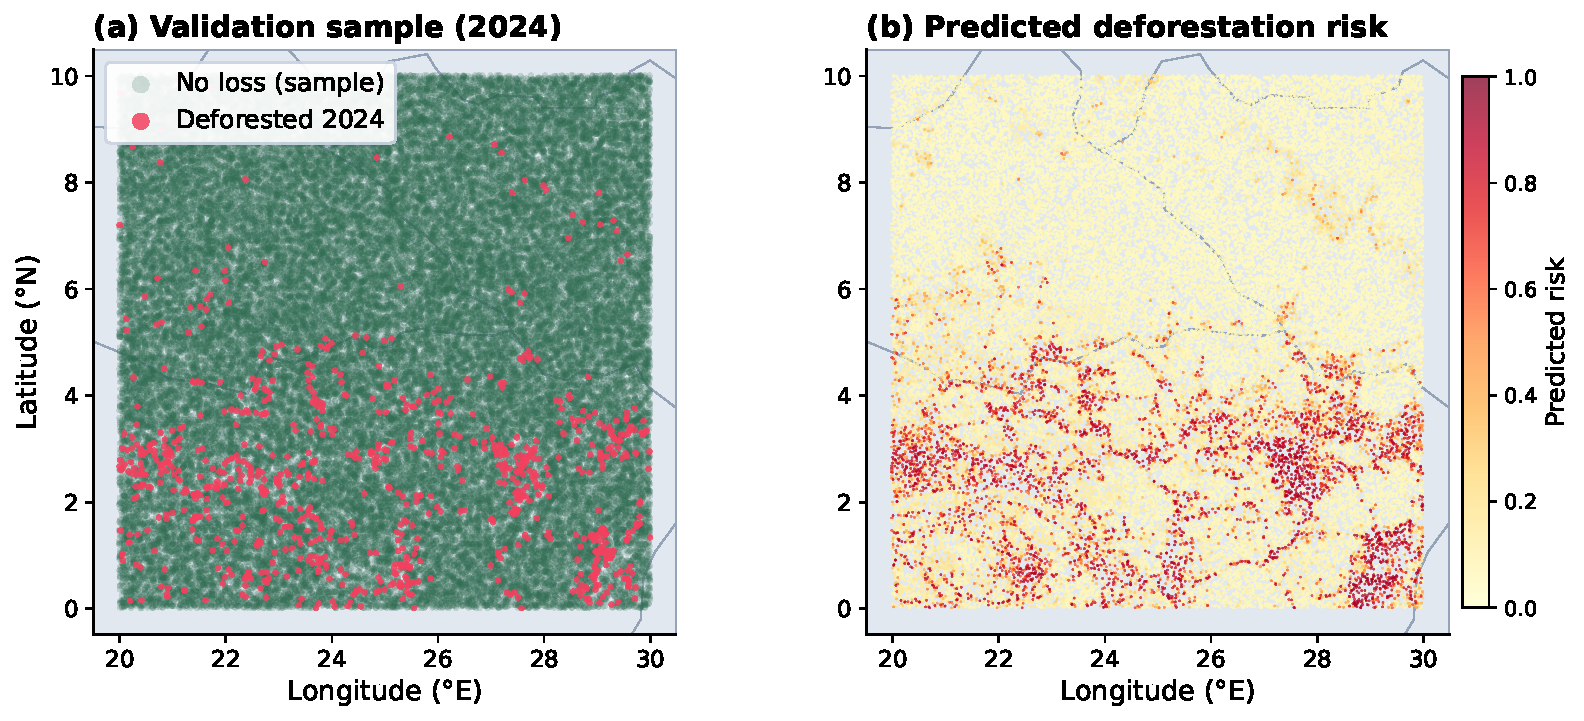
\includegraphics[width=\textwidth]{figures/fig1_study_area.pdf}
\caption{\label{fig:study_area}
(a)~Spatial distribution of the 240\,230 validation sample pixels
(2024 prediction year) over the 10°N/020°E Hansen tile.
Red dots indicate pixels that experienced tree-cover loss in 2024
(871 events, 0.36\% prevalence).
(b)~Predicted deforestation risk for the same pixels from the full 549-feature
model (AUC-ROC\,=\,0.954); this model is used for the spatial risk map
because it was deployed in the operational monitoring application.
The parsimonious 139-feature core model achieves AUC\,=\,0.955 with
higher PR-AUC (see text).
Elevated risk (orange--red) clusters along the eastern DRC forest frontier
and the Central African Republic--DRC border.
Country boundaries from Natural Earth.}
\end{figure}

\begin{figure}[htbp]
\centering
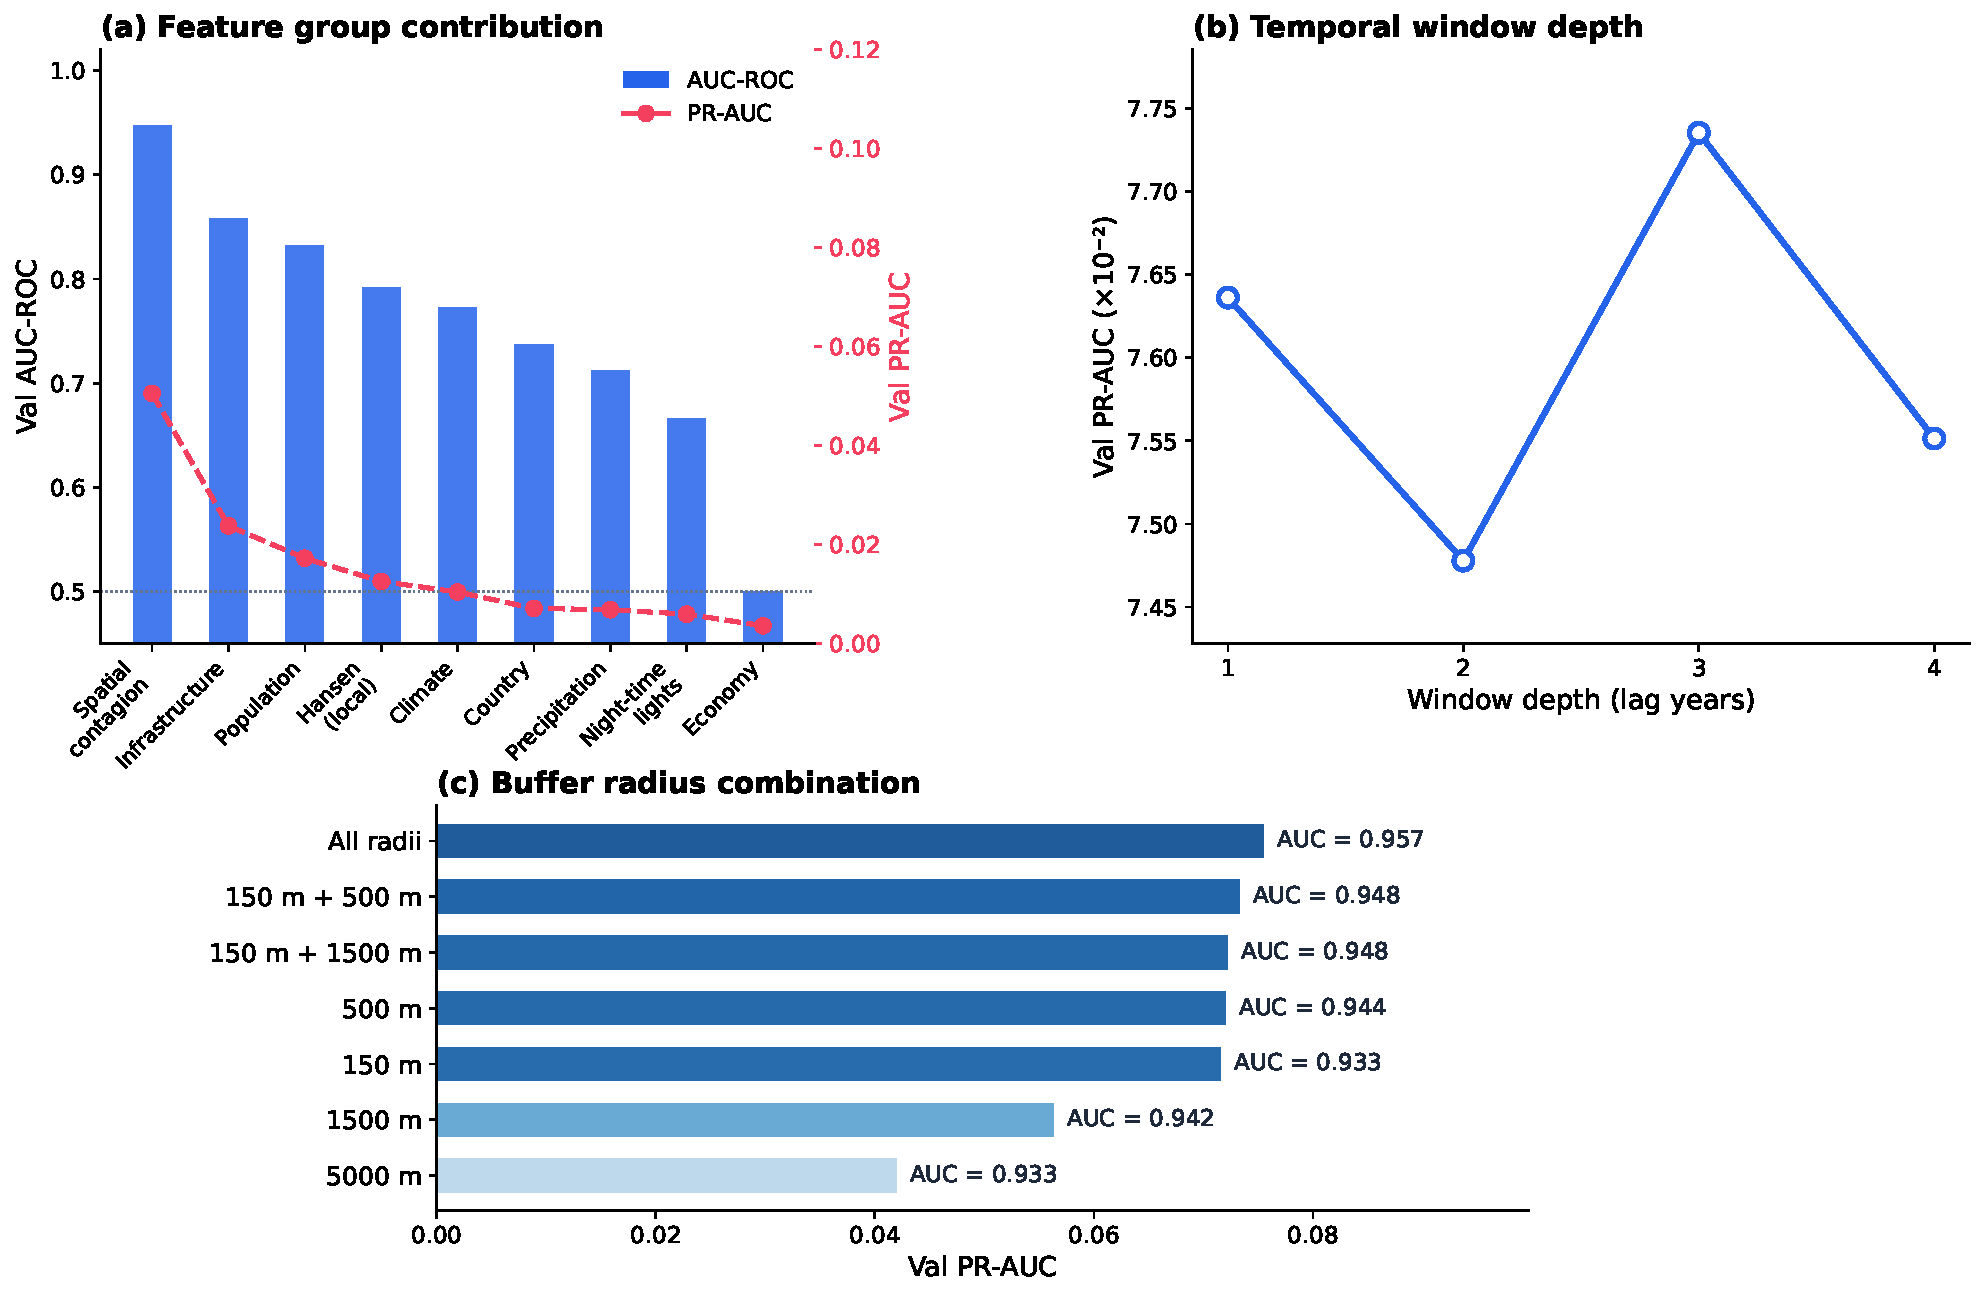
\includegraphics[width=\textwidth]{figures/fig2_ablation.pdf}
\caption{\label{fig:ablation}
Triple feature ablation results on the 2024 validation set.
(a)~Dimensional ablation: validation AUC-ROC (blue bars, left axis)
and PR-AUC (orange dots, right axis) for each feature group used alone,
ordered by single-group contribution.
(b)~Temporal ablation: PR-AUC as a function of lag-window depth
(1--4 years); the near-flat curve confirms that one lag year suffices.
(c)~Spatial ablation: PR-AUC for seven buffer-radius configurations;
AUC-ROC annotated on each bar.}
\end{figure}

\begin{figure}[htbp]
\centering
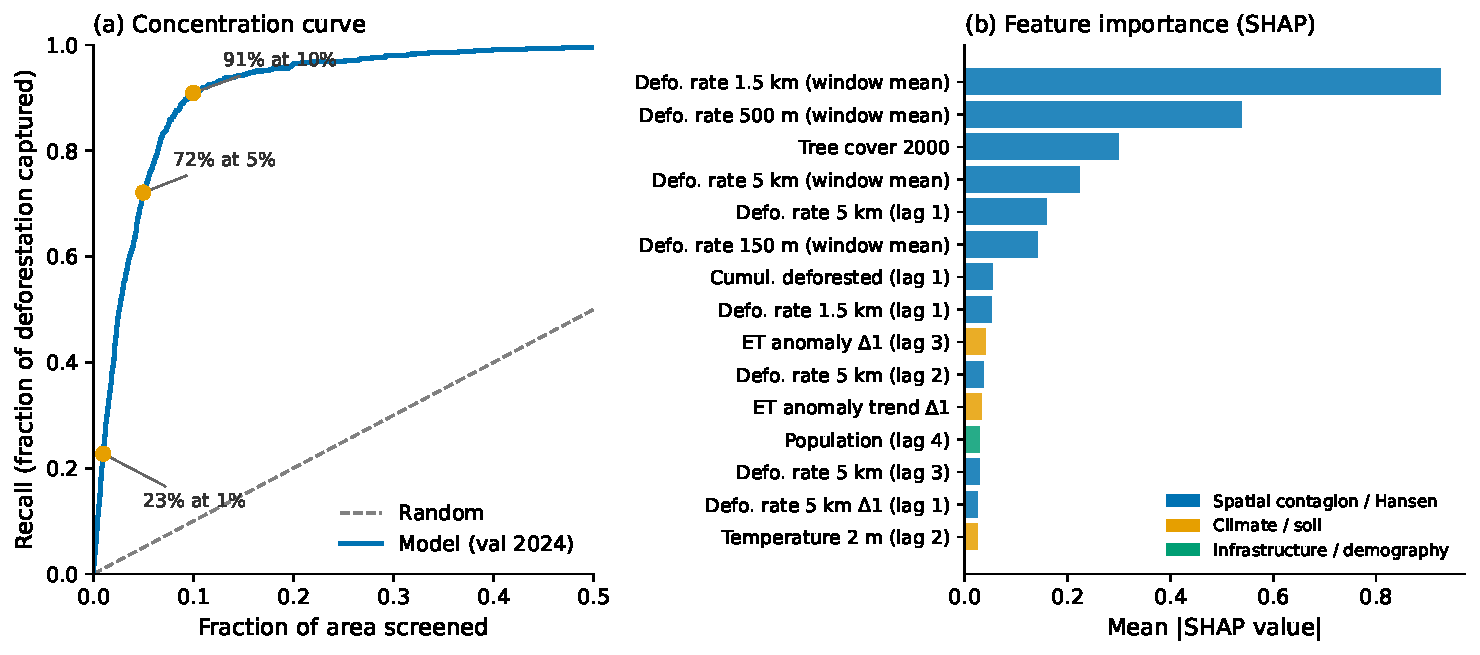
\includegraphics[width=\textwidth]{figures/fig3_lift_shap.pdf}
\caption{\label{fig:lift_shap}
(a)~Concentration curve for the deployed model on the 2024 validation set:
fraction of observed deforestation captured versus fraction of area screened.
Annotated values indicate recall at 1\%, 5\%, and 10\% screening thresholds.
The dashed line represents random screening.
(b)~Top-15 features by mean absolute SHAP value.
Bar colour encodes magnitude (sequential blue gradient: darker\,=\,higher importance).
Feature group labels (Spatial, Climate, Demography) are annotated to the right
of each bar.}
\end{figure}

\begin{figure}[htbp]
\centering
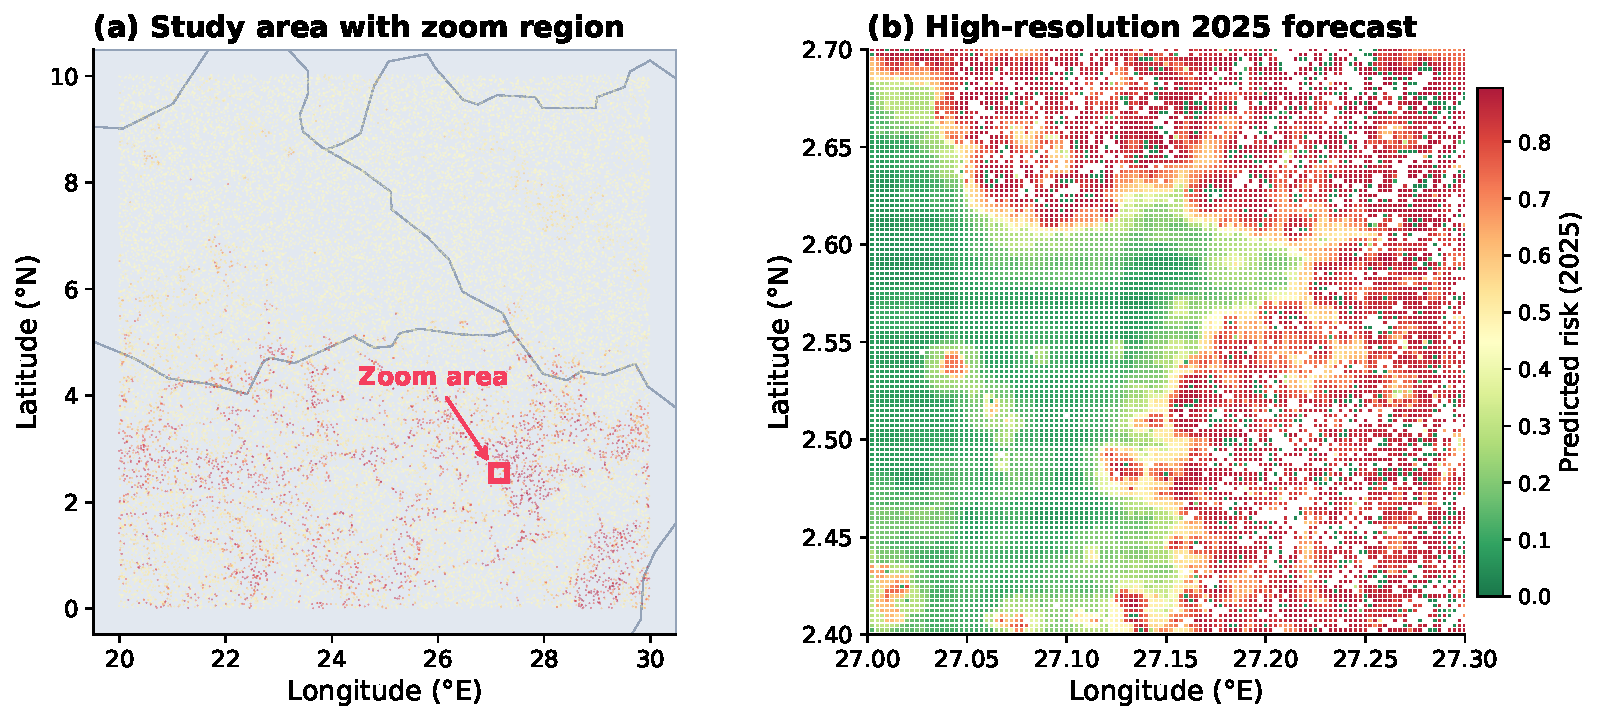
\includegraphics[width=\textwidth]{figures/fig4_demo_zone.pdf}
\caption{\label{fig:demo_zone}
High-resolution deforestation forecast for 2025.
(a)~Study area overview with the 0.3\textdegree{}\,$\times$\,0.3\textdegree{}
zoom region (red rectangle) in northeastern Congo.
(b)~Pixel-level risk map at 250\,m spacing (13{,}232~points).
Green indicates low predicted risk (intact forest); red indicates
high risk (active deforestation frontier).
This is a true forecast: no 2025 deforestation data exists at time of writing.}
\end{figure}

\end{document}
